\documentclass[]{book}
\usepackage{lmodern}
\usepackage{amssymb,amsmath}
\usepackage{ifxetex,ifluatex}
\usepackage{fixltx2e} % provides \textsubscript
\ifnum 0\ifxetex 1\fi\ifluatex 1\fi=0 % if pdftex
  \usepackage[T1]{fontenc}
  \usepackage[utf8]{inputenc}
\else % if luatex or xelatex
  \ifxetex
    \usepackage{mathspec}
  \else
    \usepackage{fontspec}
  \fi
  \defaultfontfeatures{Ligatures=TeX,Scale=MatchLowercase}
\fi
% use upquote if available, for straight quotes in verbatim environments
\IfFileExists{upquote.sty}{\usepackage{upquote}}{}
% use microtype if available
\IfFileExists{microtype.sty}{%
\usepackage{microtype}
\UseMicrotypeSet[protrusion]{basicmath} % disable protrusion for tt fonts
}{}
\usepackage[margin=1in]{geometry}
\usepackage{hyperref}
\hypersetup{unicode=true,
            pdftitle={Informatics and Statistics for Molecular Biologists (MOLB 7900)},
            pdfauthor={Jay Hesselberth},
            pdfborder={0 0 0},
            breaklinks=true}
\urlstyle{same}  % don't use monospace font for urls
\usepackage{natbib}
\bibliographystyle{apalike}
\usepackage{longtable,booktabs}
\usepackage{graphicx,grffile}
\makeatletter
\def\maxwidth{\ifdim\Gin@nat@width>\linewidth\linewidth\else\Gin@nat@width\fi}
\def\maxheight{\ifdim\Gin@nat@height>\textheight\textheight\else\Gin@nat@height\fi}
\makeatother
% Scale images if necessary, so that they will not overflow the page
% margins by default, and it is still possible to overwrite the defaults
% using explicit options in \includegraphics[width, height, ...]{}
\setkeys{Gin}{width=\maxwidth,height=\maxheight,keepaspectratio}
\IfFileExists{parskip.sty}{%
\usepackage{parskip}
}{% else
\setlength{\parindent}{0pt}
\setlength{\parskip}{6pt plus 2pt minus 1pt}
}
\setlength{\emergencystretch}{3em}  % prevent overfull lines
\providecommand{\tightlist}{%
  \setlength{\itemsep}{0pt}\setlength{\parskip}{0pt}}
\setcounter{secnumdepth}{5}
% Redefines (sub)paragraphs to behave more like sections
\ifx\paragraph\undefined\else
\let\oldparagraph\paragraph
\renewcommand{\paragraph}[1]{\oldparagraph{#1}\mbox{}}
\fi
\ifx\subparagraph\undefined\else
\let\oldsubparagraph\subparagraph
\renewcommand{\subparagraph}[1]{\oldsubparagraph{#1}\mbox{}}
\fi

%%% Use protect on footnotes to avoid problems with footnotes in titles
\let\rmarkdownfootnote\footnote%
\def\footnote{\protect\rmarkdownfootnote}

%%% Change title format to be more compact
\usepackage{titling}

% Create subtitle command for use in maketitle
\newcommand{\subtitle}[1]{
  \posttitle{
    \begin{center}\large#1\end{center}
    }
}

\setlength{\droptitle}{-2em}

  \title{Informatics and Statistics for Molecular Biologists (MOLB 7900)}
    \pretitle{\vspace{\droptitle}\centering\huge}
  \posttitle{\par}
    \author{Jay Hesselberth}
    \preauthor{\centering\large\emph}
  \postauthor{\par}
      \predate{\centering\large\emph}
  \postdate{\par}
    \date{2019-04-22}

\usepackage{booktabs}
\usepackage{amsthm}
\makeatletter
\def\thm@space@setup{%
  \thm@preskip=8pt plus 2pt minus 4pt
  \thm@postskip=\thm@preskip
}
\makeatother

\begin{document}
\maketitle

{
\setcounter{tocdepth}{1}
\tableofcontents
}
\chapter*{Course Overview}\label{course-overview}
\addcontentsline{toc}{chapter}{Course Overview}

Informatics and Statistics for Molecular Biologists (MOLB 7900) is
offered at the University of Colorado School of Medicine and teaches
students how to design and analyze common molecular biology experiments.

\chapter*{Syllabus}\label{syllabus}
\addcontentsline{toc}{chapter}{Syllabus}

\section{Course Overview}\label{course-overview-1}

Informatics and Statistics for Molecular Biologists (MOLB 7900) teaches
students to design and analyze experiments commonly used in molecular
biology. The course is organized around the Central Dogma (DNA
\textgreater{} RNA \textgreater{} Protein) wherein each block presents
2-3 experimental approaches. Each week, a new experiment is introduced
with a discussion of appropriate design and statistical considerations.
The remaining weeks' classes are devoted to digging into the analysis of
a sample data set.

The course begins with a 4 week ``boot camp'' designed to get students
familiar with and bring them up to speed on using software for shell
programming and data analysis with R and Python. We also establish
accounts on Github for problem set submission.

\subsection{Block 0: Bootcamp}\label{block-0-bootcamp}

\begin{verbatim}
A: Shell programming
B: R Studio
C: Integration with Git
D: Python
\end{verbatim}

\subsection{Block 1: DNA}\label{block-1-dna}

\begin{verbatim}
A: Chromatin accessibility
B: Motif finding
C: Variant Calling
\end{verbatim}

\subsection{Block 2: RNA}\label{block-2-rna}

\begin{verbatim}
A: Quantitative PCR
B: Bulk mRNA-seq
C: RNA-protein interaction (CLIP)
\end{verbatim}

\subsection{Block 3: PROTEIN}\label{block-3-protein}

\begin{verbatim}
A: Mass spectrometry (counts)
B: Densitometry of gel images 
C: Fluorescent protein localization (Chad)
\end{verbatim}

\section{Course Objectives}\label{course-objectives}

\begin{itemize}
\tightlist
\item
  Cater to students of many backgrounds (more computational or more
  biological)
\item
  Be able to formulate questions that are testable with computational
  techniques
\item
  Understand the limitations of sequencing-based techniques
\item
  Be fluent in statistical considerations for different approaches and
  design well-controlled experiments that can be analyzed using
  statistical tests
\item
  Be fluent in command-line programming, scripting (Python) and data
  analysis / viz (R / R Studio)
\item
  Understand the value of internet-based analysis tools (NCBI BLAST etc)
\item
  Use reproducible software development approaches (Github) and dynamic
  documents (Rmarkdown)
\item
  Independently conceive of and implement a soup to nuts reanalysis of
  an existing data set, which are presented to the class.
\end{itemize}

\section{Class Schedule}\label{class-schedule}

Monday, Wednesday, and Friday, 1-2:30pm from Sept 10 to Dec 10.

\chapter{Bootcamp}\label{bootcamp}

This 4 week ``boot camp'' is designed to get students familiar with and
bring them up to speed on using software for shell programming and data
analysis with R and Python. We also establish accounts on Github for
problem set submission.

\section{Shell programming}\label{shell-programming}

Students will become familiar with the operating in the Shell, which is
closely related to command-line/terminal. The Shell is a program which
runs other programs rather than doing calculations itself. Bash is the
default shell on most modern implementations of Unix, Mac, and in most
packages that provide Unix-like tools for Windows.

\textbf{After this section, students will be able to navigate
directories, create an organized directory structure for a project, and
install and run software.}

\section{Rstudio}\label{rstudio}

Students will learn to use \href{https://www.rstudio.com/}{Rstudio},
which is an integrated development environment that makes it way easier
to code in R. Within Rstudio, students will use
\href{https://rmarkdown.rstudio.com/}{Rmarkdown} to produce high-quality
reports, presentations, and documents in a highly reproducible manner.
Students will become fluent in importing, processing, and transforming
data using a collection of R packages designed for data science
\href{https://www.tidyverse.org/}{tidyverse}.

\begin{center}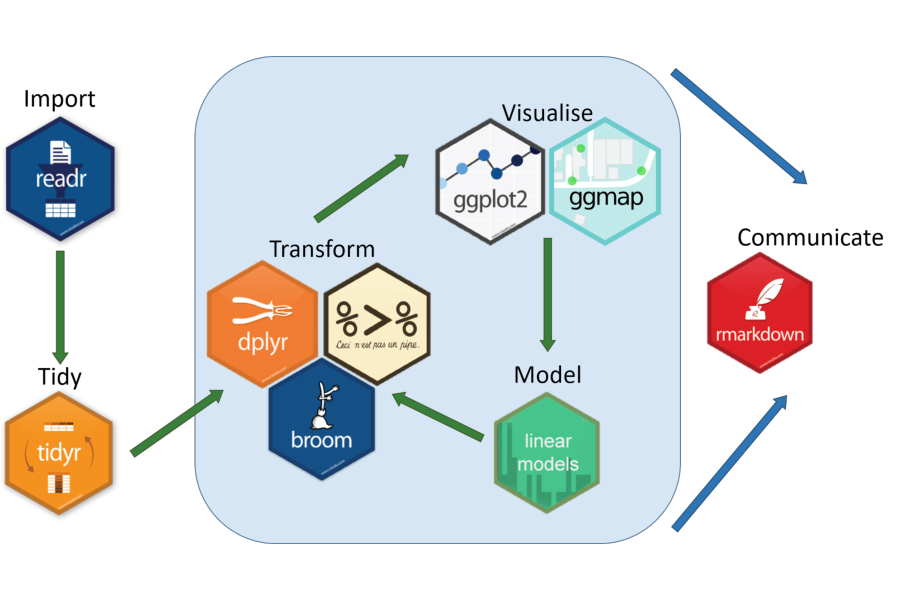
\includegraphics{Informatics_and_Statistics_for_Molecular_Biologists_files/figure-latex/unnamed-chunk-1-1} \end{center}

After achieving exellence in basic data handling, students will be
introduced to a broad range of commonly used statistical tests and an
underlying conceptual framework for deciding the appropriate statistical
test. We will emphasize concepts unique to genomic/big data. These
statistical concepts and tests will be revisited during applied sections
of the course in which specific technology and data are introduced and
re-analyzed.

\textbf{After this section, students will be able to import, process,
transform, visualize data; use statistical tests to analyze basic
tabular data; genarate html/pdf reports of their work.}

\section{Git}\label{git}

Modern scientists need to write code as part of their research. This
code needs to be documented just as bench experiments need to be logged
in a lab notebook. Version control systems like
\href{https://git-scm.com}{Git}, and online hosting site,
\href{https://github.com}{GitHub}, are critical tools to address these
important issues. These tools allow students to track iterative changes
made to their code, revert to a specific previous version, and share
their code with the broader scientific community. Altogether these tools
are a cornerstone of reproducible research practices that is
conveniently integrated within Rstudio and Rmarkdown.

\textbf{After this section, students will be able to use git within
Rstudio to easily version and share their code. They will be expected to
turn in assignments using git in Rstudio.}

\section{Python}\label{python}

\href{https://www.python.org/}{Python} is an easy to learn language that
combines the flexibility of bash along with the conveniences of higher
level languages like R. This useful for solving problems for which
software does not exist, which is important for students to learn in
order to anticipate unmet needs and data from new technologies/assays.
Many tools for the analysis of modern datasets are available as python
packages, allowing the incorporation of pre-built analysis tools within
custom, made-from-scratch, code. Furthermore, python's suitability as a
scripting language makes it a natural fit for APIs of other common
analysis tools. For example, image analysis pipelines can be constructed
in \href{https://imagej.net/Jython_Scripting}{Fiji}, allowing the batch
processing of many files at once.

\textbf{After this section, students will be able to write basic
software and scripts that will enable them to derive meaning from the
large datasets typical of modern biology.}

\chapter{Block 1: DNA}\label{block-dna}

\chapter{Block 2: RNA}\label{block-rna}

\chapter{Block 3: Protein}\label{block-protein}

\chapter{Exercises}\label{exercises}

\bibliography{book.bib,packages.bib}


\end{document}
